\documentclass[a4paper,11pt,notitlepage,hidelinks]{article}

\usepackage{ucs}
\usepackage[utf8x]{inputenc}
\usepackage{amsmath}
\usepackage{amsfonts}
\usepackage{amssymb}
\usepackage{amsthm}
\usepackage{caption}
\usepackage{subfigure}
\usepackage{wrapfig}
\usepackage{fullpage}
\usepackage[usenames]{xcolor}
\usepackage[english]{babel}
\usepackage[T1]{fontenc}
\usepackage{placeins}
\usepackage[pdftex]{graphicx}
\usepackage[pdftex]{hyperref}
\usepackage{tikz}
\usepackage{multicol}
\usepackage[noend,linesnumbered,noresetcount]{algorithm2e}

\usetikzlibrary{calc,decorations.markings,arrows}

\author{Jan Kończak}
\title{JPaxos results}
\date{12.09.2013}

\begin{document}

% Text width: \the\textwidth

All-test setup, unless onterwise specified:
\begin{itemize}
 \item 3 replicas on \texttt{hpc\{2..4\}}
 \item 3×500 clients on \texttt{hpc\{5..7\}}
 \item default properties (tcp, window size=2)
 \item no-op logging
 \item 1kB request size
\end{itemize}

Code base: commit 5617bc047f0660d05f14b87b1e42f163d5b248ae



\section{CPU or network saturation}

Target: see what is the bottleneck in JPaxos - network or CPU?

Measured: cpu and network usage on leader, follower and client machine.

\subsection{1024B requests}

\subsubsection{CPU}
\strut

Iddle CPU on nodes [percentage]:\\
{\ttfamily
\begin{tabular}{|r|c|c|c|}\hline
/ & Client & Follower & Leader \\ \hline
0 & 89,60  & 69,57    & 58,67  \\ \hline
1 & 89,16  & 80,12    & 57,95  \\ \hline
2 & 86,34  & 89,32    & 67,76  \\ \hline
3 & 64,52  & 60,87    & 37,45  \\ \hline
\end{tabular}         
}

\medskip

Leader and follower average CPU detailed usage:\\
{\ttfamily
\begin{tabular}{|c|c|c|c|c|c|c|}\hline
          &  user  &   sys  & iowait & irq   & soft  & idle  \\ \hline
leader:   & 23,92  &  10,13 & 0,07   & 1,77  & 8,66  & 55,46 \\ \hline
follower: & 14,51  &  04,71 & 0,12   & 1,06  & 4,62  & 74,97 \\ \hline
\end{tabular}
}

\medskip

Leader per-core CPU detailed usage:\\
{\ttfamily
\begin{tabular}{|c|c|c|c|c|c|c|c|}\hline
CPU & user   & sys   & iowait& irq  &  soft  &  idle  \\ \hline
0   & 31,25  & 8,27  & 0,00  & 0,00 &  1,81  &  58,67 \\ \hline
1   & 30,08  & 9,55  & 0,00  & 0,00 &  2,42  &  57,95 \\ \hline
2   & 18,26  & 11,22 & 0,00  & 0,00 &  2,76  &  67,76 \\ \hline
3   & 16,09  & 11,47 & 0,28  & 7,06 &  27,66 &  37,45 \\ \hline
\end{tabular}
}

\medskip

{\small Legend:\\
\begin{tabular}{rl}
user & executing at the user level (application)\\
 sys & executing at the system level (kernel) without any interrupts\\
 irq & hardware interrupts\\
soft & software interrupts\\
\end{tabular}
}

\paragraph{Conclusions}
CPU is not saturated.
Thread CPU usage is unbalanced.
Thread performing network tasks uses processor at most.
If the throughput would increase by 60\%, the CPU would be a possible bottleneck.

New test needed: how small must the request size be to saturate CPU.

\subsubsection{Network}

Used bandwidth on nodes [10\textasciicircum 6bits/s aka Mbit/s]:

\begin{tabular}{|r|c|c|c|}\hline
 /  & Client & Follower & Leader \\ \hline
in  & 130    & 484      & 394    \\ \hline
out & 128    & 215      & 908    \\ \hline
\end{tabular}

Measured TCP throughput on the network is 941.07 [10\textasciicircum 6bits/s] (3× \texttt{netperf -H hpc3 -cC -fm -j -tTCP\_STREAM -\strut- -m 1024}).
Bandwidth used during the test TCP throughput test is 987 [10\textasciicircum 6bits/s].

\paragraph{Conclusions}
Network usage reaches 92\% of its capabilities. This means that the network is close to saturation, yet not fully saturated.
Network is a bottleneck in this test.

% TODO: request size / bandwidth

\subsection{Multiple request sizes}

Following test shows how JPaxos behaves with 16B, 128B, 1024B and 8196B requests.\\
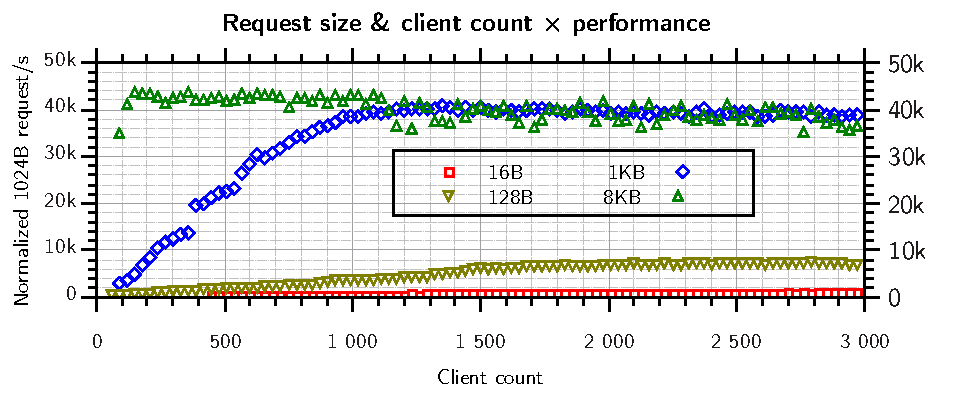
\includegraphics{varia/reqSize-cliCount}

The values on the plot are normalized, i.e., 8KB request count per second has been multiplied by 8, and the 128B request count per second has been divided by 8. This makes the results comparable.

With 8KB requests the network gets saturated very soon (with 150 clients).
With 1KB requests the network gets saturated starting from 1200 clients.
Smaller requests cannot saturate the network, and after reaching peek throughput at about 2500 clients, the performance drops.

\bigskip

To see when the border request byte size where JPaxos stops saturating CPU and starts saturating network, the following test has been done:
 \begin{itemize}
 \item 3×700 clients
 \item request size varying from 16B to 2048B
\end{itemize}

The results, unnormalized, are as follows:\\
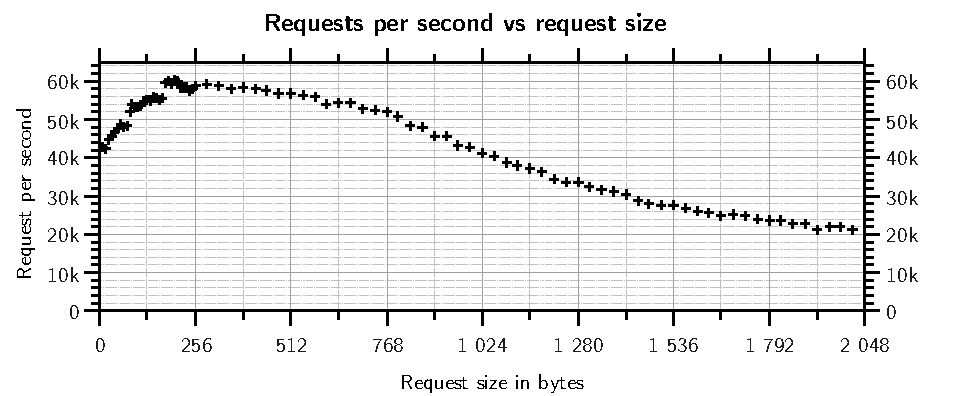
\includegraphics{varia/reqSize_reqs.pdf}

So to get highest request per second value (in order to show 'we have the highest r/s'), one must take 200B requests.
This however says nothing about real performance.

\medskip

Following plot shows state-machine level goodput (i.e. how much data the state machine got in a time unit):\\
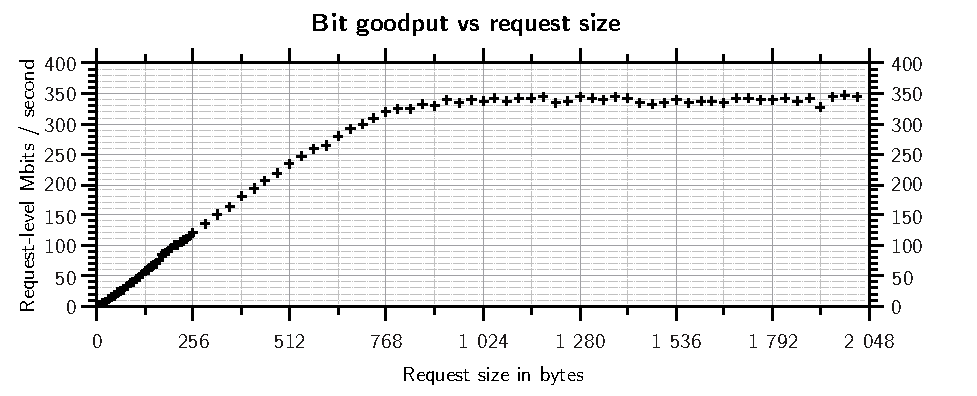
\includegraphics{varia/reqSize_mbps.pdf}

The plot shows that when the request size exceeds about 900B, the network gets saturated. 
Up to 768 bytes the bit throughput grows nearly linearly with increasing request size -- larger request takes the same CPU time, but transports more data. Starting from about 900B the number of requests per second decreases, but the amount of data remains on a stable level, indicating ghat the network bandwidth limits throughput.

The test included 2100 clients total, which is enough to produce an amount of request needed to saturate the network from clients to the replicas starting with request size of 180B (in theory), so increasing the number of client won't change the 
900B limit.


\subsection{200B requests}

After analysing various request sizes, 200B requests were taken under account:

\subsubsection{Network}

Used bandwidth on nodes [10\textasciicircum 6bits/s aka Mbit/s]:\\
\begin{tabular}{|r|c|c|c|}\hline
 /  & Client & Follower & Leader \\ \hline
in  & 57     & 172      & 136    \\ \hline
out & 52     & 99       & 297    \\ \hline
\end{tabular}

There is a lot of bandwidth free. Less than 1/3rd of bandwidth is used on any machine in any single direction. Network is not the bottleneck.

\subsubsection{CPU}

Iddle CPU on nodes [percentage]:\\
{\ttfamily
\begin{tabular}{|r|c|c|c|}\hline
/ & Client & Follower & Leader \\ \hline
0 & 81,66  & 50,03    & 43,72  \\ \hline
1 & 82,75  & 54,90    & 36,86  \\ \hline
2 & 79,96  & 81,70    & 62,68  \\ \hline
3 & 55,98  & 68,00    & 46,98  \\ \hline
\end{tabular}         
}

All machines have higher CPU usage, but there is still a lot of free time on any node. (?)

\medskip

Leader and follower average CPU detailed usage:\\
{\ttfamily
\begin{tabular}{|c|c|c|c|c|c|c|}\hline
          &  user  &   sys  & iowait & irq   & soft  & idle  \\ \hline
leader:   & 33,09  & 12,12  & 0,09   & 0,83  & 6,16  & 47,4  \\ \hline
follower: & 24,86  &  7,63  & 0,17   & 0,51  & 3,17  & 63,66 \\ \hline            
\end{tabular}
}

\medskip

Leader per-core CPU detailed usage:\\
{\ttfamily
\begin{tabular}{|c|c|c|c|c|c|c|c|}\hline
CPU & user   & sys   & iowait& irq  &  soft  & idle  \\ \hline
0   & 39,13  & 15,63 & 0,00  & 0,00 &  1,50  & 43,74 \\ \hline
1   & 51,78  & 10,23 & 0,00  & 0,00 &  1,07  & 36,91 \\ \hline
2   & 24,30  & 11,43 & 0,00  & 0,04 &  1,43  & 62,80 \\ \hline
3   & 17,14  & 11,18 & 0,35  & 3,36 & 20,95  & 47,03 \\ \hline
\end{tabular}
}

Leader has a lot to do, but there is free processor time left.

If not CPU and network, it seems that synchronisation issues slow down the JPaxos now. (I hope to have time to discuss it with Tadek and Maciej). 
\section{Choosing window size}

Nuno in [Tuning Paxos for high-throughput with batching and pipelining] stated that:
\begin{quotation}
A note on the cluster results: In the experiments performed in a cluster environment, batching by itself is enough to achieve the maximum throughput, with pipelining having minimal impact on the results. The reason for this difference is that the latency in a cluster is very low so the leader does not have time to start new instances while waiting for the results of previous instances.
\end{quotation}
This is however false. (At least on HPC cluster.)

During the tests first window size 1÷5 has been tested, showing that the higher window size, the better the results are:\\
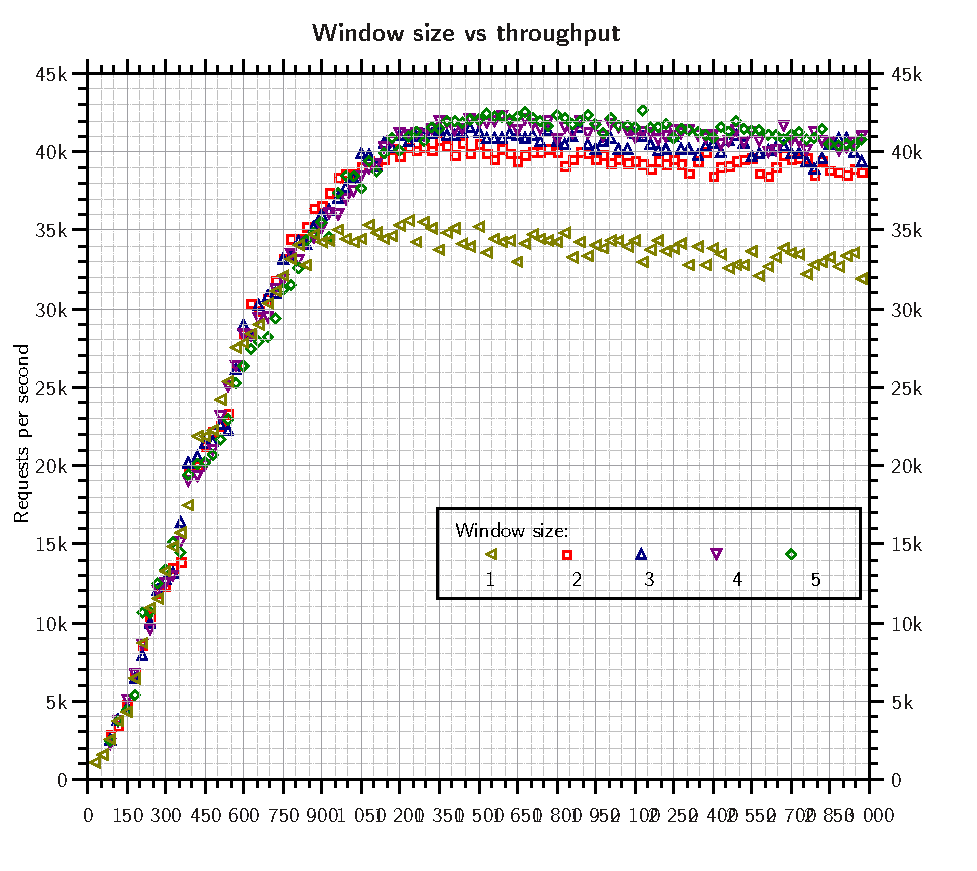
\includegraphics{varia/ws.pdf}

The tests have been continued up to window size 10, as the performance increase stabilized at window size 6 and higher.
To present the results in more readable way, the points represent the gain (in \%) from the worst result at each client count:\\
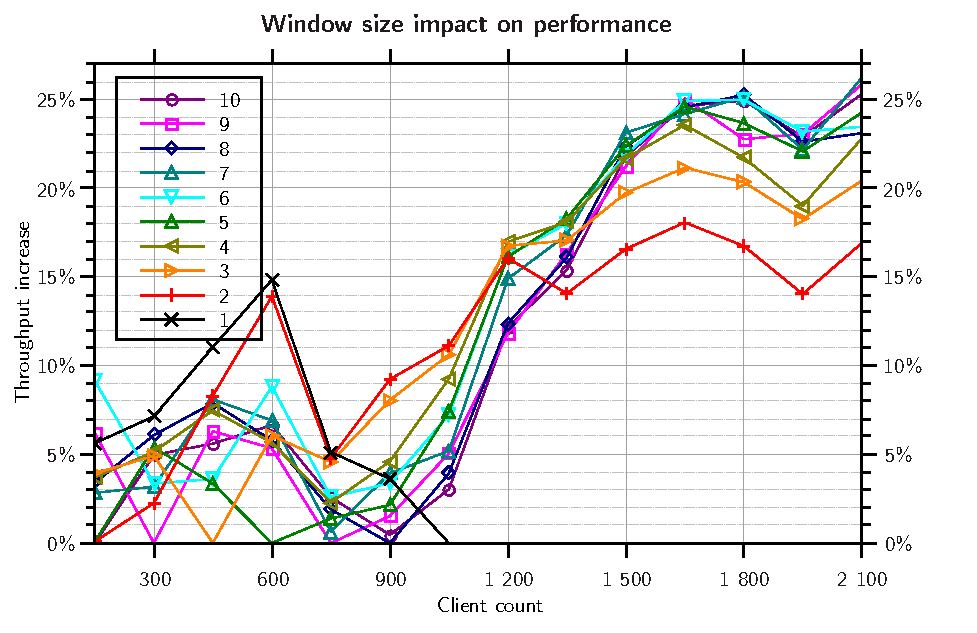
\includegraphics{varia/ws_2d.pdf}

To make the results even more readable (at least for me) the performance gain has been also presented on a 3d plot -- x and y axes represent client count and window size accordingly, while the colour - the brighter the better - represents performance gain:\\
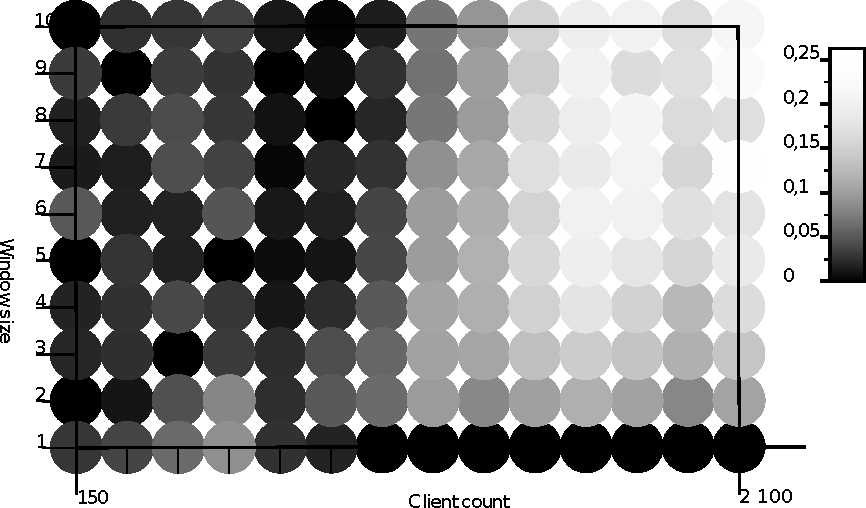
\includegraphics{varia/ws_3d.pdf}

What is not presented on the plots is the variance of the results. As for each client count and window size JPaxos has been run 10 times, except from bare performance also the variance of the performance can be calculated. The results are presented below -- \emph{notice:} the color scale is not linear this time \\
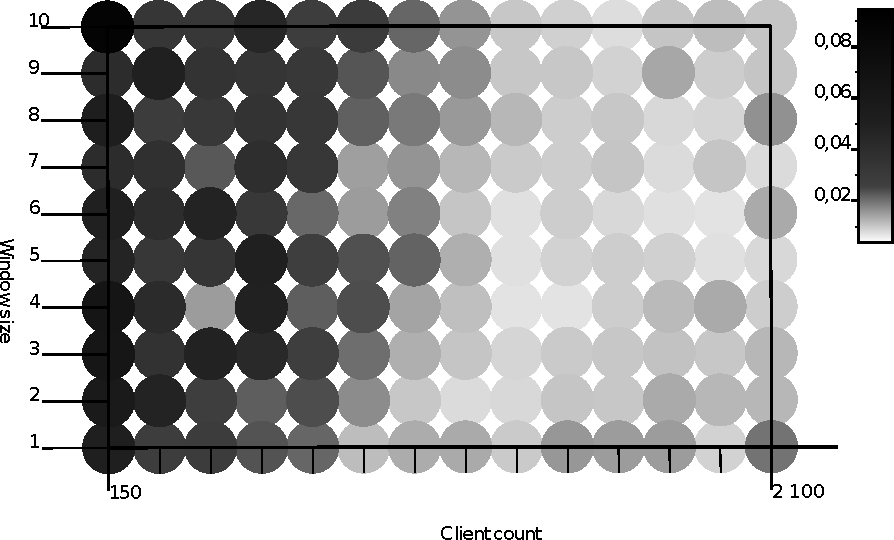
\includegraphics{varia/ws_3d_dev.pdf}

As long as the network is not saturated, the throughput is not stable; after the network becomes the bottleneck, the results are rather stable.

\paragraph{Conclusions}
The window size (and whole pipelining optimisation) is also important on cluster environments, increasing the speed in critical cases by 25\% compared to no pipelining. As long as the network is not saturated, the result stdev is about 5\%, and the gains are in order of 5\% as well. On one hand, this makes choosing right window size hard, on the other -- the performance loss on wrong choice is not big. After saturating the network pipelining increases the performance a lot. Also the stdev drops to 1\%, making the results easier repeatable.

The window size of 6 and higher seems to be the best choice. It is advised to keep the window size as low as possible (due to its negative impact on the speed of recovering from any failures, i.e., view change and recovery). So proper window size for HPC cluster at tests with 1kB requests is six. 


\section{NIO network implementation impact on performance}

Maciej and Tadek extended JPaxos by new implementation of Network module -- NIO. They expected NIO to be faster than 'old' java IO (which we call TCP, despite both Network modules using TCP). These tests show if it was worth writing.

\subsection{1024B requess -- network saturation}

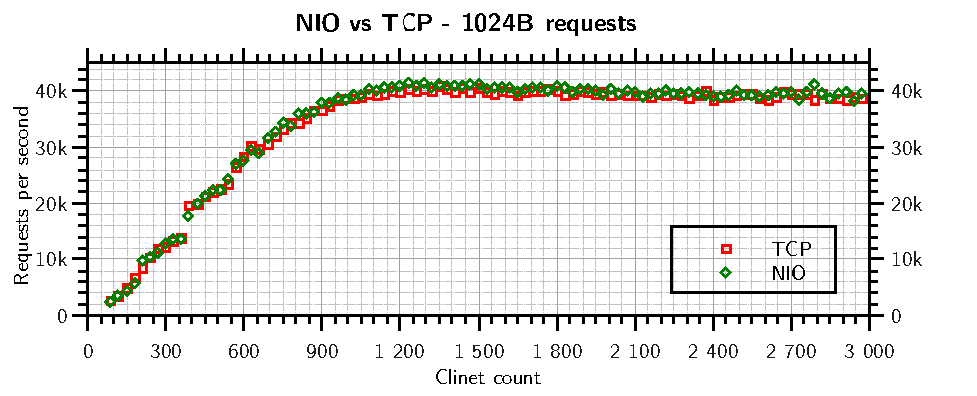
\includegraphics{tcp_nio/tcp_nio_1024}

NIO throughput is 'a little better' -- on average higher by 0,7\%. The trend is identical.

\subsection{128B requess -- CPU saturation}

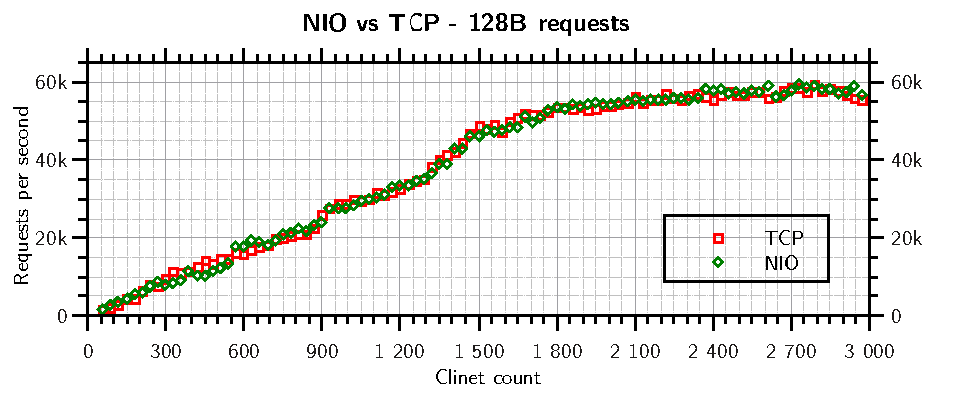
\includegraphics{tcp_nio/tcp_nio_128}

Here, the CPU is more saturated. NIO was meant to help in such case. The experiments however do not agree with this claim -- NIO and 'old IO' perform the same (NIO is on average 0,3\% slower).

\paragraph{Conclusion} it makes no real difference for JPaxos whether it uses NIO or 'old IO'. 
\section{Logging impact on performance}

Using standard logging facility is flexible and cost-efficient method for analysing the behaviour of systems like JPaxos.
However, logging takes some CPU time, and therefore may impact results.
Previous JPaxos version used \texttt{java.util.logging} (JUL) for logging, which -- as most built-in Java mechanisms -- is rather performance-unfriendly.
Now JPaxos uses \texttt{slf4j} with \texttt{logback} backend, and two classes of messages are tagged with marks: logging all performance-related events and logging recovery events only.
Slf4j (contrary to java.util.logging) can be turned off at all (i.e. there is no effective logging code). Logback can as well as JUL suppress all messages, makes it however a lot faster.

Tests how much recording events affects performance are presented here:\\
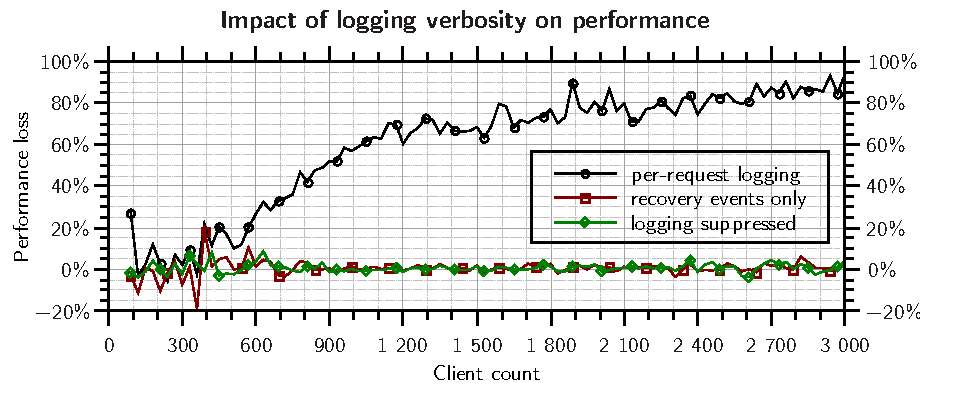
\includegraphics{varia/log_impact.pdf}

Test for each parameter values have been performed once only, however total of 100 tests for different client count are enough to take general conclusions. First, no-op logging is faster than suppressing all logging by 6‰, faster than selecting recovery-related events by 5‰, and faster than logging all performance-related events by 60\%. This means that using logging for recording recovery-related events has little impact on performance and can be used in benchmarks, while full logging on request basis cannot.
Also, full logging cost increases with client count (what is quite obvious, more clients = more requests to trace).
The results for tests up to 900 clients have big variations (what is normal for JPaxos in such case), but the trends remain unaffected. 

\end{document}
